\documentclass{ximera}
\graphicspath{{./content/01_5_graphing/graphics/}{./graphics/}}
\title{Graphing Functions}
\begin{document}
\begin{abstract}
\end{abstract}
\maketitle

In this section, we'll cover some approaches for graphing multivariable functions $\mathbb{R}^n\rightarrow\mathbb{R}$, focusing on the case where $n=2$. Before we define the graph of such a function, let's think about how we graph a single variable function.

Consider the function $f(x) = x^2$, which is a function $f:\mathbb{R}\rightarrow\mathbb{R}$. The graph of this function is the set of all points $(x,x^2)$ in the $xy$-plane, and we draw this graph below.


We get this set of points by taking each possible input, $x\in\mathbb{R}$, with its corresponding output, $x^2\in\mathbb{R}$. We then plot this point in the $xy$-plane. So the graph will include points $(1,1), (2,4), (\sqrt{pi}, \pi)$, and so on. Notice that for this function, which has domain $\mathbb{R}$ and codomain $\mathbb{R}$, the graph is a subset of $\mathbb{R}^2$. We'll keep this in mind as we turn our attention to multivariable functions.

\section*{Definition of the Graph of a Function}

You might already have an intuitive idea of what the graph of a function $f:X\subset\mathbb{R}^2\rightarrow\mathbb{R}$ should be, but perhaps don't know the formal definition, or how to figure out what the graph of an arbitrary function looks like. We'll begin with the definition of the graph, before discussing how to actually produce graphs.

\begin{definition}
Let $f:X\subset\mathbb{R}^n\rightarrow\mathbb{R}$ be a function. The \emph{graph} of $f$ is the set of points
\[
\textrm{Graph }f = \{(\vec{x},f(\vec{x})\,:\,\vec{x}\in X\}
\]
in $\mathbb{R}^{n+1}$.

When $n=2$, we typically visualize a point in the graph as lying over the point $\vec{x}$ in the plane at a height $f(\vec{x})$.
\end{definition}

Note that this is similar to the graph of a function from a subset of $\mathbb{R}$ to $\mathbb{R}$: for each input in $\mathbb{R}^n$, we group it with its output (which is a point in $\mathbb{R}$), to obtain a point in $\mathbb{R}^{n+1}$.

\begin{example}
Consider the function $f:\mathbb{R}^2\rightarrow\mathbb{R}$ defined by $f(x,y) = x^2$. The graph of this function is the following surface in $\mathbb{R}^3$.

\begin{image}
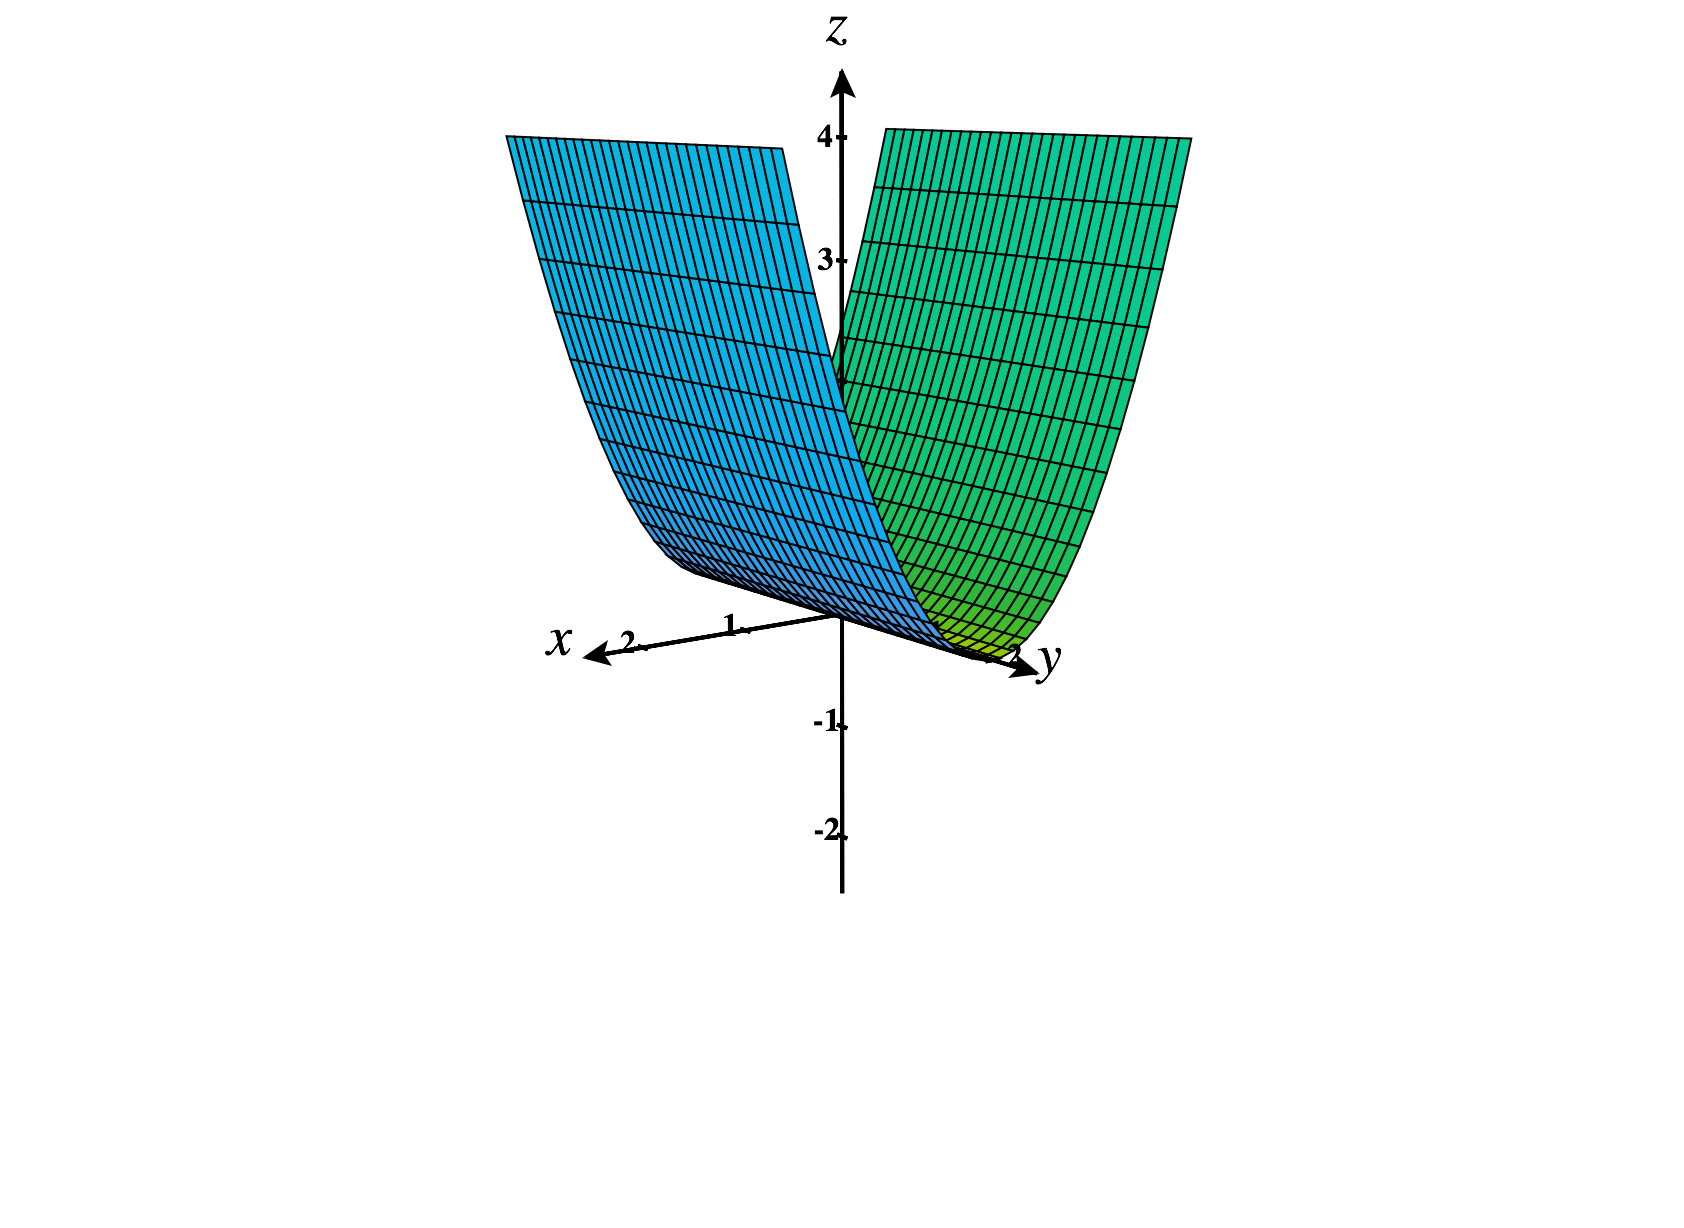
\includegraphics[width = \textwidth]{CalcPlot3D-x2}
\end{image}
\end{example}

\section*{Strategies for Graphing}

For now, we'll focus on graphing functions $f:X\subset\mathbb{R}^2\rightarrow\mathbb{R}$. It can be much trickier to sketch the graph of such a function than it was to sketch the graphs of functions $\mathbb{R}\rightarrow\mathbb{R}$, especially since we'll often be trying to represent a three-dimensional object in a two-dimensional image. One common strategy that people will initially try is plotting individual points to try to get a sense of the graph. However, for graphs in $\mathbb{R}^3$, you would need a lot of points to get a representative sample of points. For this reason, \emph{plotting points alone is not an effective strategy}. However, plotting a single point here or there can be helpful.

We've now told you what doesn't work for graphing functions in $\mathbb{R}^3$, so now we should probably figure out what does work. The essential idea of all of these strategies is that we know you're pretty comfortable graphing single variable functions in $\mathbb{R}^2$, so we're going to take advantage of that experience.

We'll begin with contour curves, which are obtained by setting the $z$-coordinate to be constant. Think of this as taking horizontal slices of the graph.

\begin{definition}
Let $f:X\subset\mathbb{R}^2\rightarrow\mathbb{R}$ be a function. The \emph{contour curve} of the function $f$ at height $C$ is the set of points in $\mathbb{R}^3$ obtained by taking the intersection of the graph of $f$ with the plane $z=C$.
\end{definition} 

\begin{example}
Consider the function $f(x,y) = x^2+y^2$. We'll find the contour curves of this function at heights $-1$, $0$, $1$, $2$, $3$, and $4$.

At height $-1$, we have the set of points $(x,y,-1)$ such that $x^2+y^2=-1$. Since squares are always nonnegative, there are no such points. So, the contour curve at height $-1$ is the empty set.

At height $0$, we have the set of points $(x,y,0)$, such that $x^2+y^2=0$. This only happens when $x=y=0$. So the contour curve at height $0$ is just the set consisting of a single point, $(0,0,0)$.

At height $1$, we have the set of points $(x,y,1)$ such that $x^2+y^2=1$. We can recognize this as a circle of radius $1$.

At height $2$, we have the set of points $(x,y,2)$ such that $x^2+y^2=2$. We can recognize this as a circle of radius $\sqrt{2}$.

At height $3$, we have the set of points $(x,y,3)$ such that $x^2+y^2=3$. We can recognize this as a circle of radius $\sqrt{3}$.

At height $4$, we have the set of points $(x,y,4)$ such that $x^2+y^2=4$. We can recognize this as a circle of radius $2$.

We plot all of these contour curves below.

\begin{image}
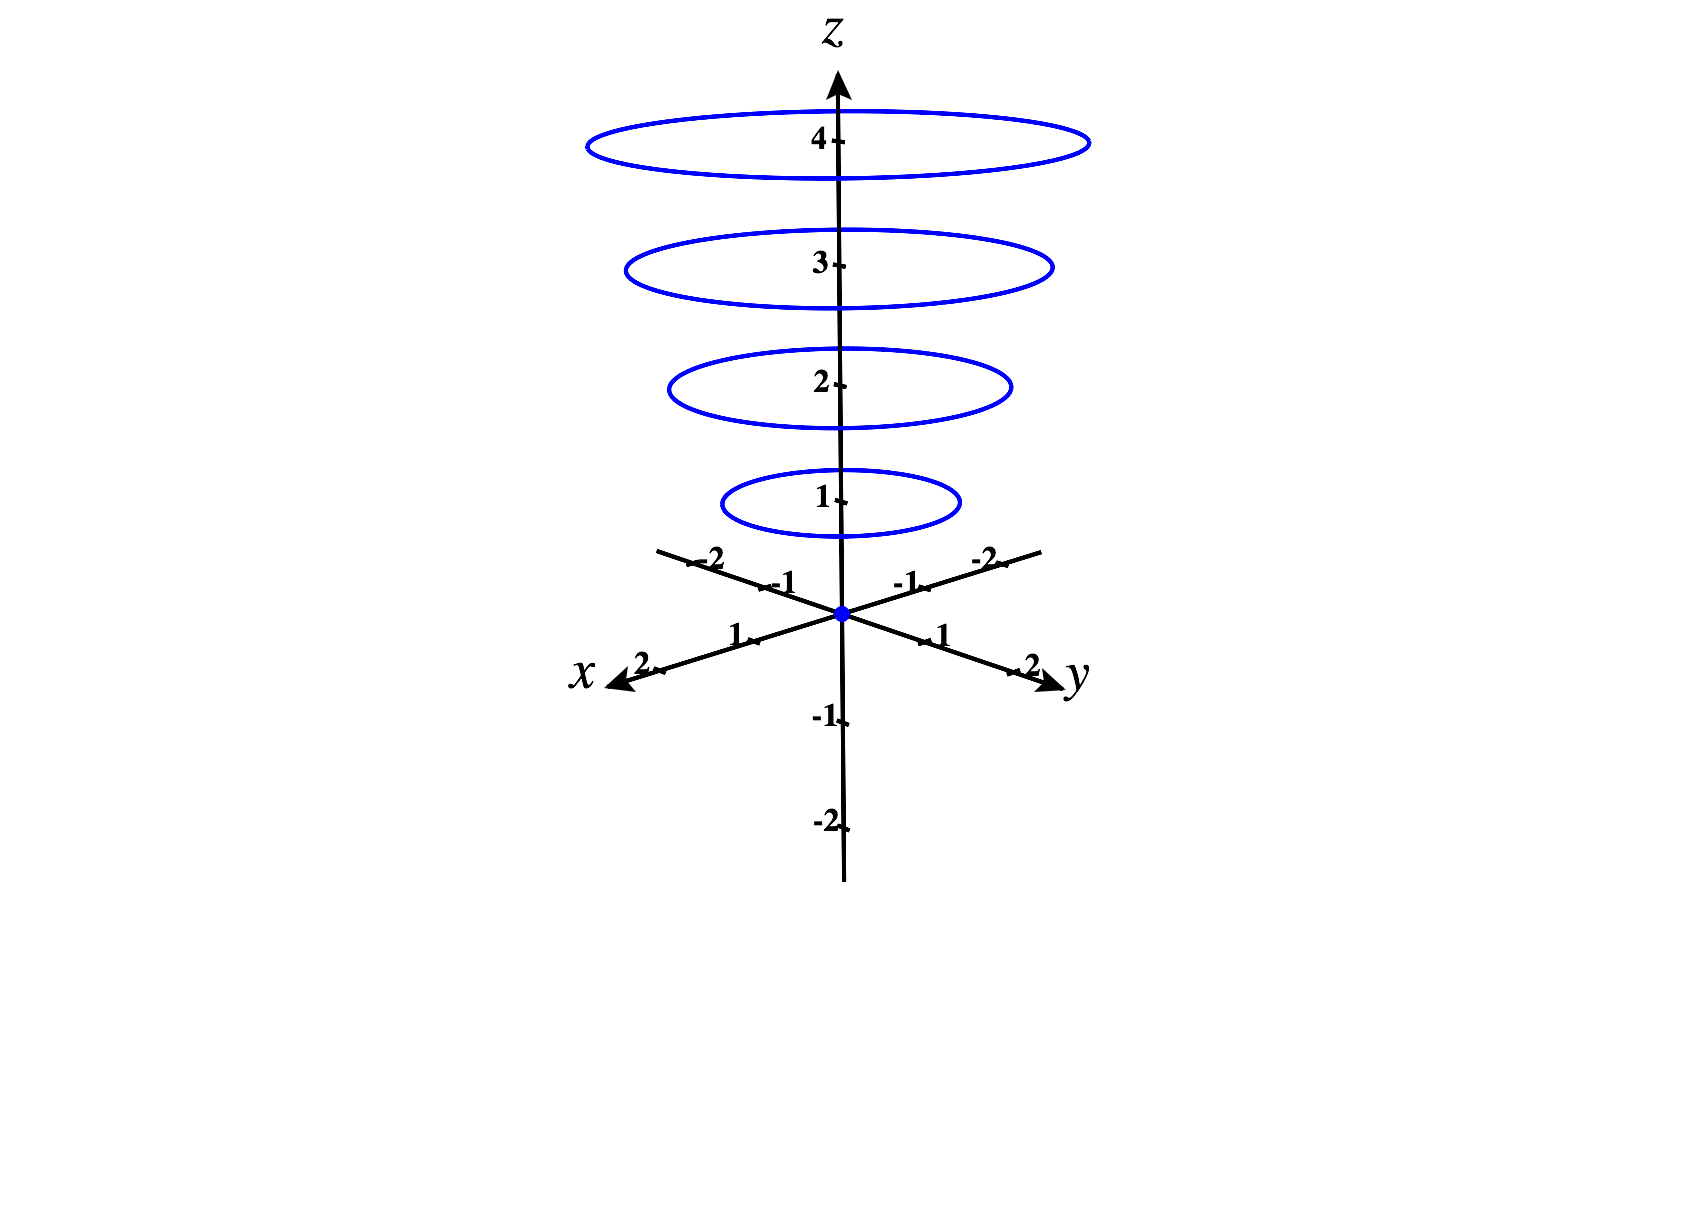
\includegraphics[width = \textwidth]{CalcPlot3D-contour}
\end{image}

Notice how these give us a sense of the graph of the function, included below.

\begin{image}
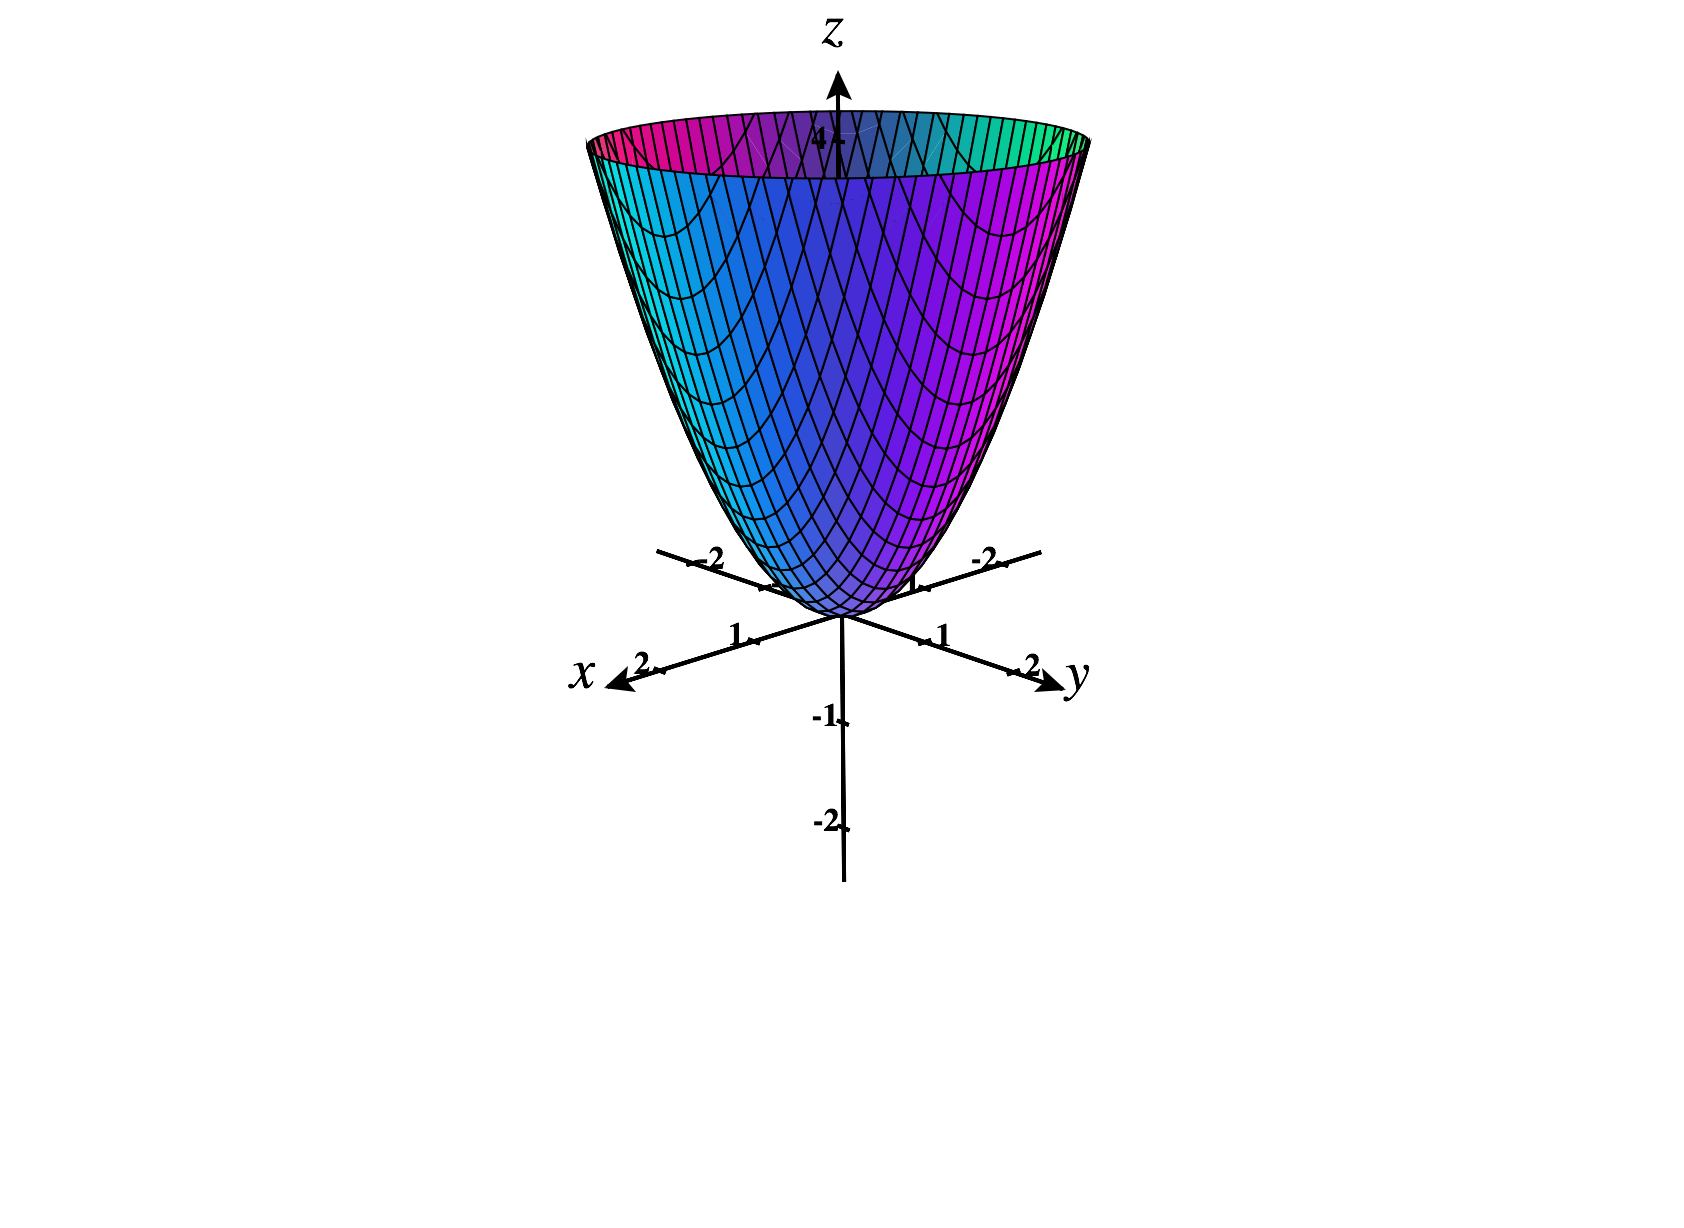
\includegraphics[width = \textwidth]{CalcPlot3D-x2plusy2}
\end{image}
\end{example}

We can also consider the level curves of a function, which are closely related to contour curves.

\begin{definition}
Let $f:X\subset\mathbb{R}^2\rightarrow\mathbb{R}$ be a function. The \emph{level curve} of the function $f$at height $C$ is the set of points in $\mathbb{R}^2$ satisfying $C = f(x,y)$.
\end{definition}

After reading this definition, you're probably thinking ``Hey, aren't contour curves and level curves the exact same thing?'' They're certainly closely related. The key difference is that level curves exist in the plane, $\mathbb{R}^2$, while contour curves exist in three-space, $\mathbb{R}^3$. Since they're in the plane, level curves are usually easier to draw. However, contour curves are more useful for figuring out the shape of a graph. For these reasons, it can be useful to go back and forth between level curves and contour curves.

\begin{example}
Consider the function $f(x,y) = x^2+y^2$. We'll find the level curves of this function at heights $-1$, $0$, $1$, $2$, $3$, and $4$.

At height $-1$, we have the set of points $(x,y)$ such that $x^2+y^2=-1$. Since squares are always nonnegative, there are no such points. So, the contour curve at height $-1$ is the empty set.

At height $0$, we have the set of points $(x,y)$, such that $x^2+y^2=0$. This only happens when $x=y=0$. So the contour curve at height $0$ is just the set consisting of a single point, $(0,0,0)$.

At height $1$, we have the set of points $(x,y)$ such that $x^2+y^2=1$. We can recognize this as a circle of radius $1$.

At height $2$, we have the set of points $(x,y)$ such that $x^2+y^2=2$. We can recognize this as a circle of radius $\sqrt{2}$.

At height $3$, we have the set of points $(x,y)$ such that $x^2+y^2=3$. We can recognize this as a circle of radius $\sqrt{3}$.

At height $4$, we have the set of points $(x,y)$ such that $x^2+y^2=4$. We can recognize this as a circle of radius $2$.

We plot all of these level curves below.

\begin{image}
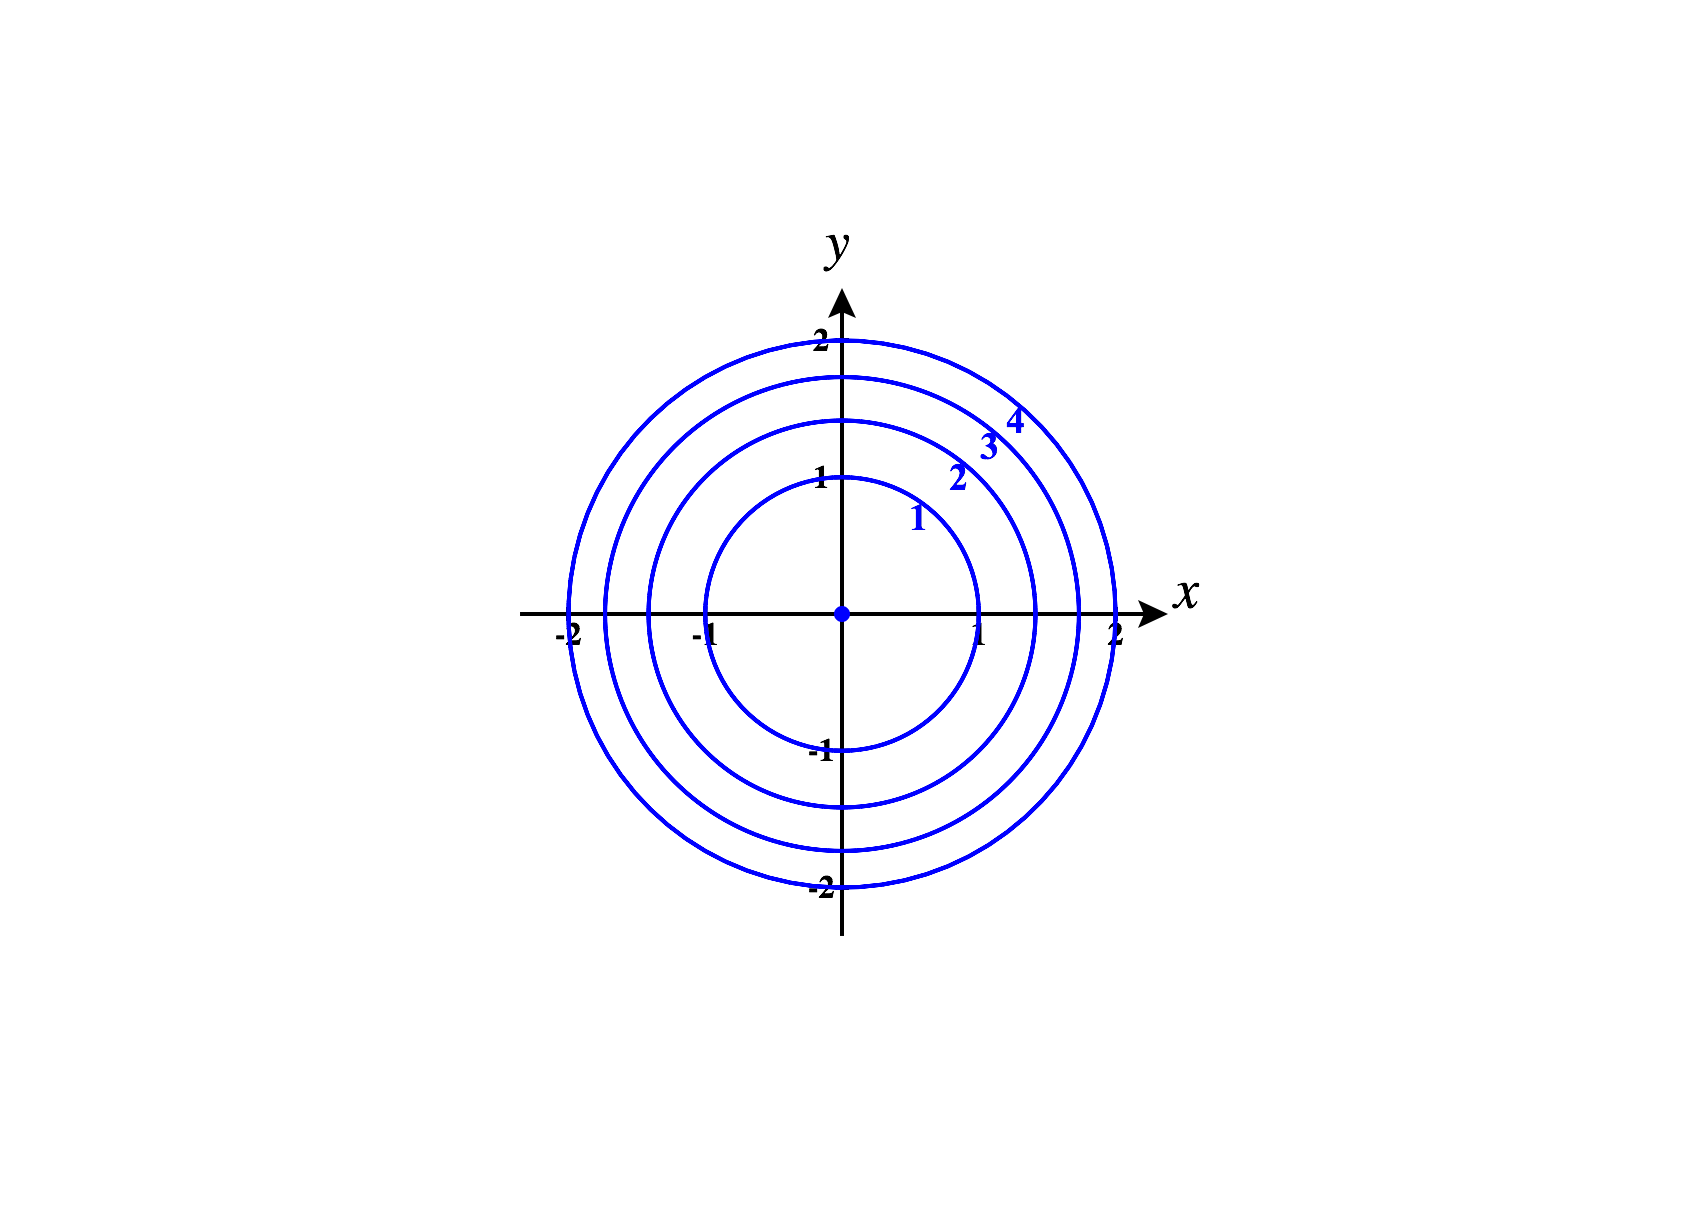
\includegraphics[width = \textwidth]{CalcPlot3D-level_sets}
\end{image}

Notice that we've labeled each level curve with its height, to help us keep track of how these curves relate to the graph of the function $f$.
\end{example}

We can think of contour curves as taking slices of the graph where $z$ is constant. It can also be useful to take slices of the graph where $x$ or $y$ is constant. We call these slices sections of the graph.

\begin{definition}
Let $f:X\subset\mathbb{R}^2\rightarrow\mathbb{R}$ be a function, and let $C$ be a constant.

The \emph{section} of the graph of $f$ by $x=C$ is the set of points 
\[
\{(C,y,z)\in\mathbb{R}^3\,:\,z = f(C,y)\}.
\]

The \emph{section} of the graph of $f$ by $y=C$ is the set of points 
\[
\{(x,C,z)\in\mathbb{R}^3\,:\,z = f(x,C)\}.
\]
\end{definition}

Note that, like contour curves, sections exist in $\mathbb{R}^3$.

\begin{example}
Consider again the function $f(x,y) = x^2+y^2$.

We'll find the sections by $x=-1$, $x=0$, and $x=1$, and by $y=-1$, $y=0$, and $y=1$.

For the section by $x=-1$, we have the set of points $(-1,y,z)$, where $z=(-1)^2+y^2=y^2+1$. We can recognize this as a parabola with vertex $(-1,0,1)$.

For the section by $x=0$, we have the set of points $(0,y,z)$, where $z=(0)^2+y^2=y^2$. We can recognize this as a parabola with vertex $(0,0,0)$.

For the section by $x=1$, we have the set of points $(1,y,z)$, where $z=(1)^2+y^2=y^2+1$. We can recognize this as a parabola with vertex $(1,0,1)$.

We graph these three sections below.

\begin{image}
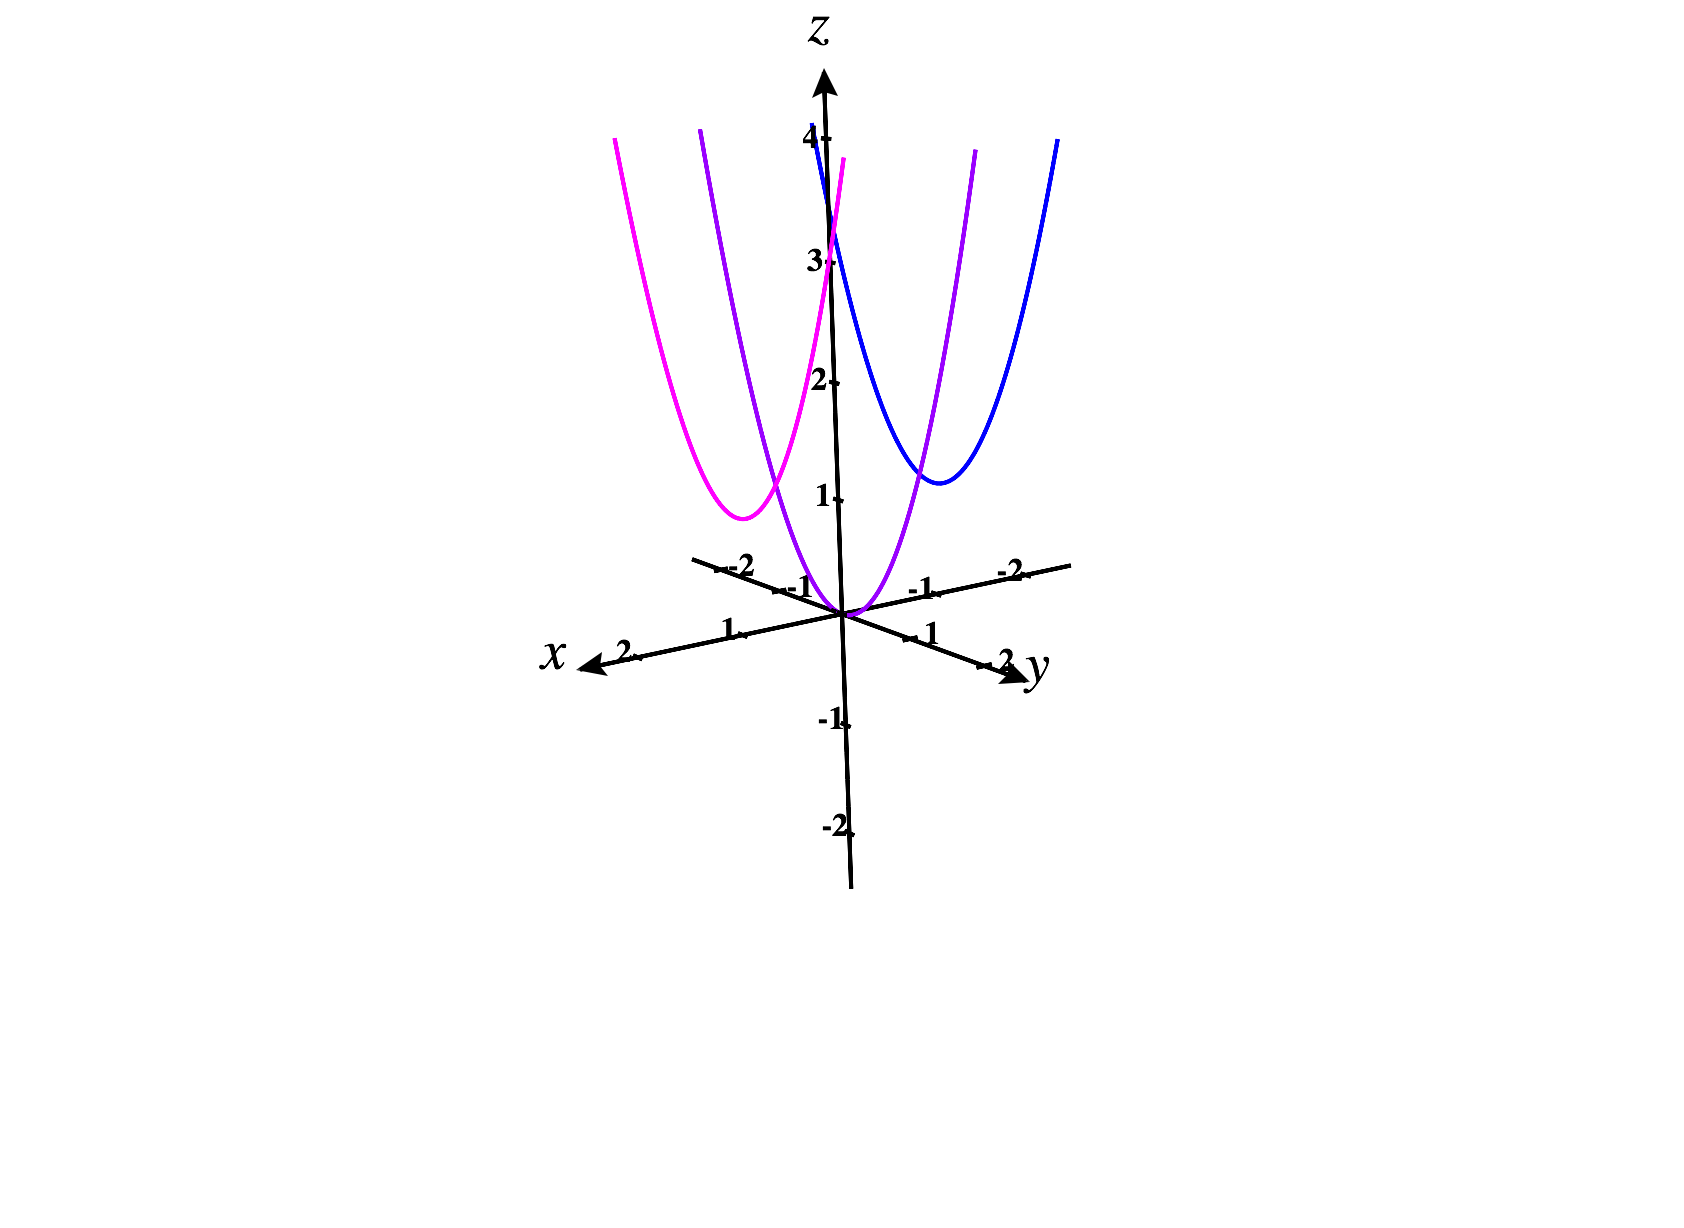
\includegraphics[width = \textwidth]{CalcPlot3D-x_sections}
\end{image}

For the section by $y=-1$, we have the set of points $(x,-1,z)$, where $z=x^2+(-1)^2=x^2+1$. We can recognize this as a parabola with vertex $(0,-1,1)$.

For the section by $y=0$, we have the set of points $(x,0,z)$, where $z=x^2+(0)^2=x^2$. We can recognize this as a parabola with vertex $(0,0,0)$.

For the section by $y=1$, we have the set of points $(x,1,z)$, where $z=x^2+(1)^2=x^2+1$. We can recognize this as a parabola with vertex $(0,1,1)$.

We graph these three sections below.

\begin{image}
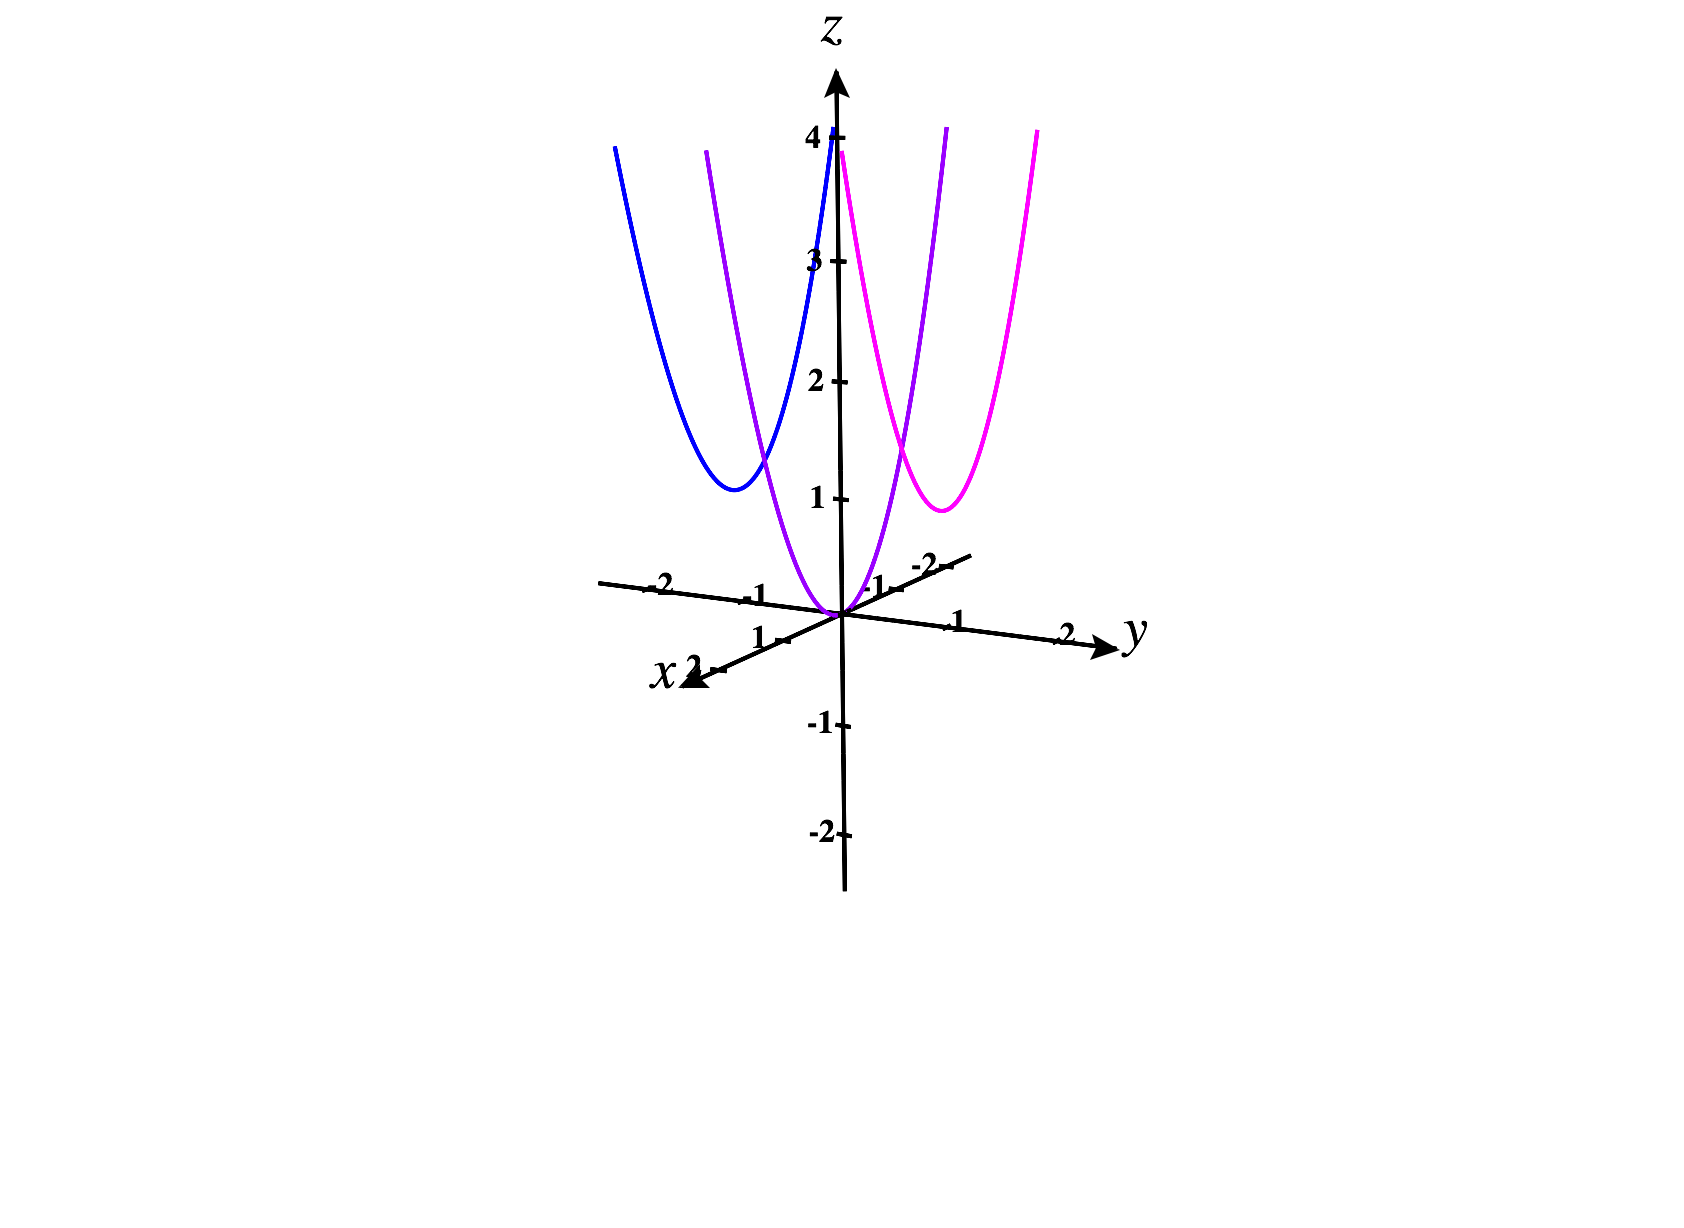
\includegraphics[width = \textwidth]{CalcPlot3D-y_sections}
\end{image}

\end{example}

\section*{Level Surfaces}

So far, we have focused on graphing functions from subsets of $\mathbb{R}^2$ to $\mathbb{R}$, so the graphs are in $\mathbb{R}^3$.

We now turn our attention to the graphs of functions from subsets of $\mathbb{R}^3$ to $\mathbb{R}$. Note that the graph of such a function will exist in $\mathbb{R}^4$. Since the world we live in only has three physical dimensions, it can be very difficult to visualize a four dimensional object! Fortunately, there are various tricks that can be used to get some sense of what a four dimensional object looks like. We cover one of them here.

When we had a function $f:D\subset\mathbb{R}^2\rightarrow\mathbb{R}$, we could get a sense of the graph by looking at its level curves, which were curves in the same plane.

For a function $f:D\subset\mathbb{R}^3\rightarrow\mathbb{R}$, we can adopt a similar approach. We can once again consider the level sets, which are obtained by taking the output to be some constant:
\[
f(x,y,z) = C.
\]
In this case, the level sets will be level surfaces, which live in $\mathbb{R}^3$. By graphing several level surfaces, we can see what a slice of the graph of $f$ looks like at various heights, giving us some sense of how the overall graph behaves. Of course, because this graph exists in four dimensions, we still probably won't be able to visualize this perfectly.

To see how this can help us visualize the four-dimensional graph of a function $f:\mathbb{R}^3\rightarrow\mathbb{R}$, we give an example.

\begin{example}
Consider the function
\[
f(x,y,z) = \sqrt{x^2 + y^2 + z^2}.
\]
Find the level surfaces at heights $-1$, $0$, $1$, $2$, and $3$. Use these level surfaces to describe the graph of $f$.

We'll begin with the level surface at height $-1$. This is the set of points $(x,y,z)$ in $\mathbb{R}^3$ such that
\[
-1 = \sqrt{x^2+y^2+z^2}.
\]
There are no points that satisfy this equation, so the level surface is empty.

Now we'll consider the level surface at height $0$. This is the set of points $(x,y,z)$ in $\mathbb{R}^3$ such that
\[
0 = \sqrt{x^2+y^2+z^2}.
\]
The only point which satisfies this equation is the origin, so the level ``surface'' is the single point $(0,0,0)$.

Let's look at the level surface at height $1$. This is the set of points $(x,y,z)$ in $\mathbb{R}^3$ such that
\[
1 = \sqrt{x^2+y^2+z^2}.
\]
Squaring both sides, we can rewriting this as 
\[
1 = x^2+y^2+z^2.
\]
The graph of this equation is the sphere of radius $1$ centered at the origin, which is our level surface.

Let's look at the level surface at height $2$. This is the set of points $(x,y,z)$ in $\mathbb{R}^3$ such that
\[
2 = \sqrt{x^2+y^2+z^2}.
\]
Squaring both sides, we can rewriting this as 
\[
4 = x^2+y^2+z^2.
\]
The graph of this equation is the sphere of radius $2$ centered at the origin, which is our level surface.

Let's look at the level surface at height $3$. This is the set of points $(x,y,z)$ in $\mathbb{R}^3$ such that
\[
3 = \sqrt{x^2+y^2+z^2}.
\]
Squaring both sides, we can rewriting this as 
\[
9 = x^2+y^2+z^2.
\]
The graph of this equation is the sphere of radius $3$ centered at the origin, which is our level surface.

In the image below, we take advantage of graphing software, and use some transparency to view these as nested spheres. In many cases, it's more clear to graph level surfaces individually. This is especially true if you're drawing the surfaces by hand.

\begin{image}
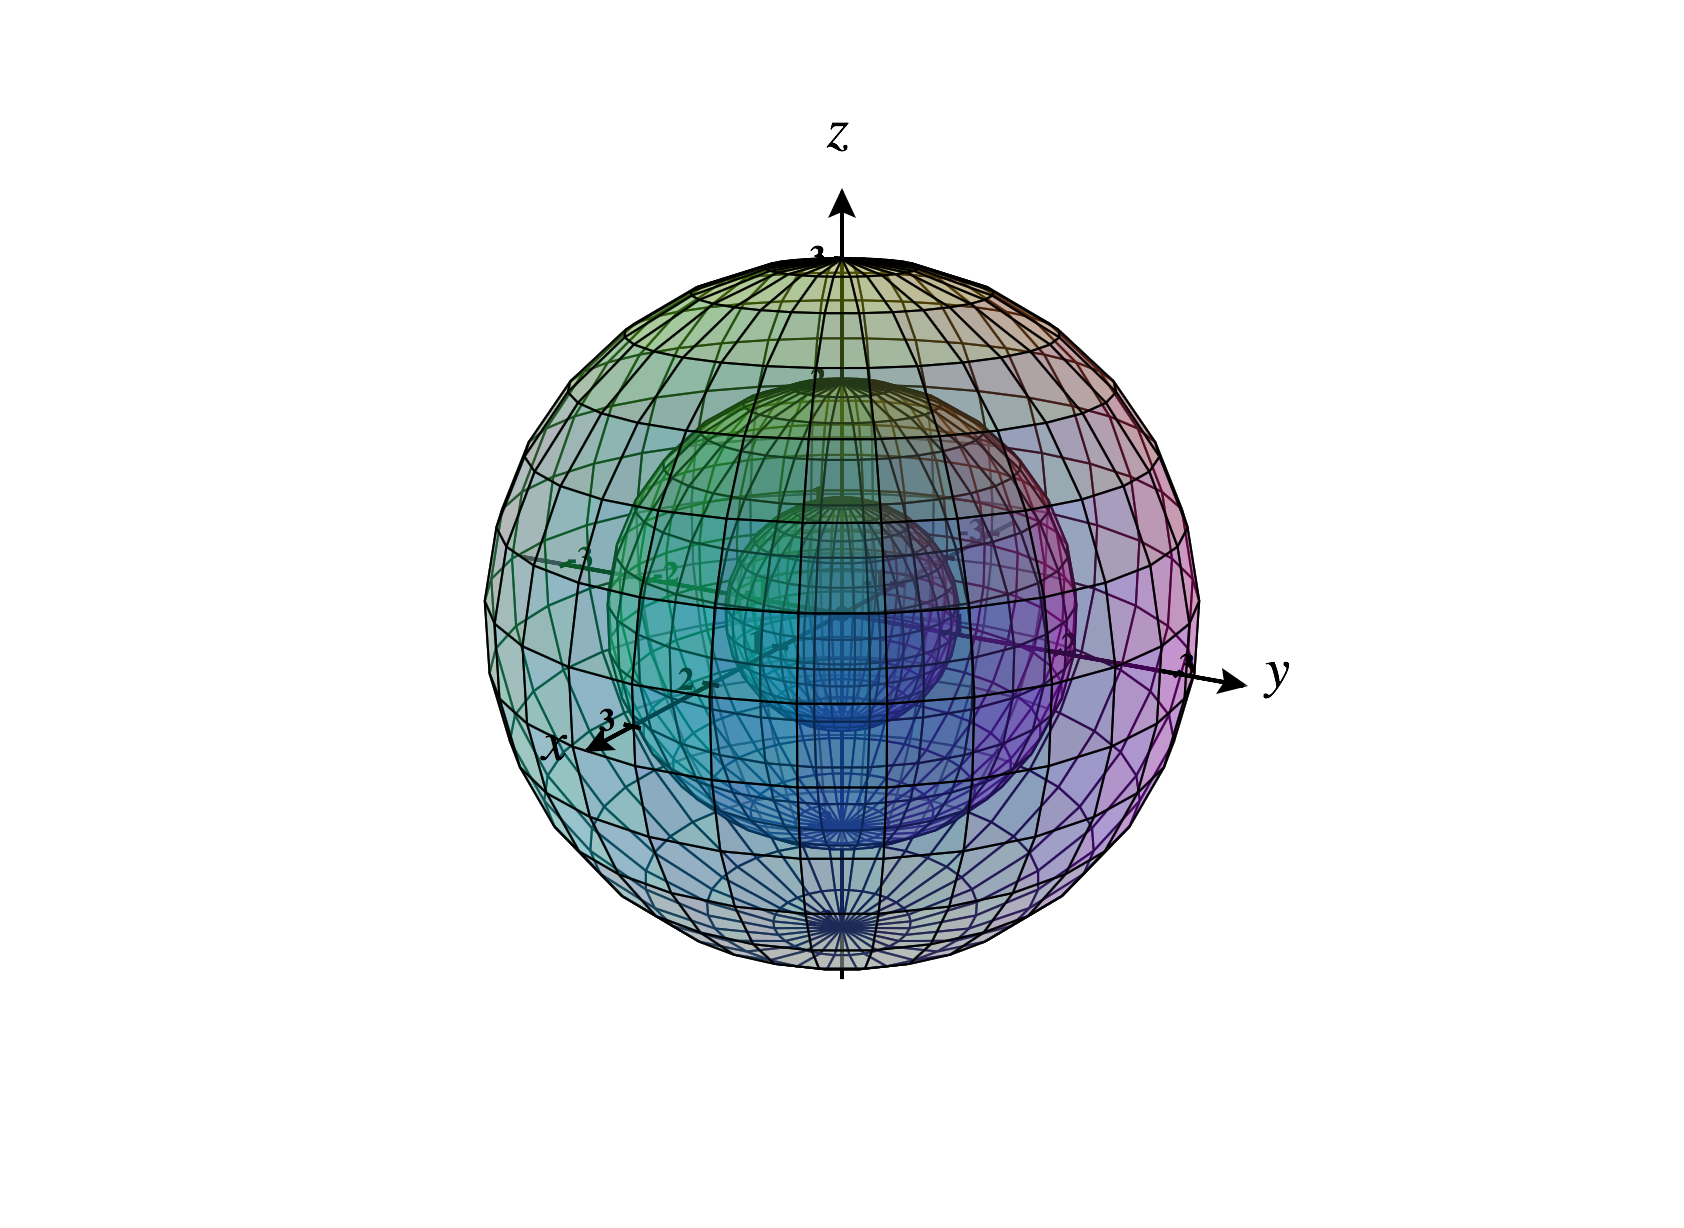
\includegraphics[width = \textwidth]{CalcPlot3D-nested_level_surfaces}
\end{image}

We can see that the level surfaces are spheres whose radii increase linearly with the height. So, we can describe the graph of $f$ as some sort of four-dimensional cone.

\end{example}



\end{document}